\documentclass[a4paper,11pt]{article}
\usepackage{amsmath,amsthm,amsfonts,amssymb,amscd,amstext,vmargin,graphics,graphicx,tabularx,multicol} 
\usepackage[francais]{babel}
\usepackage[utf8]{inputenc}  
\usepackage[T1]{fontenc} 
\usepackage{pstricks-add,tikz,tkz-tab,variations}
\usepackage[autolanguage,np]{numprint} 

\setmarginsrb{1.5cm}{0.5cm}{1cm}{0.5cm}{0cm}{0cm}{0cm}{0cm} %Gauche, haut, droite, haut
\newcounter{numexo}
\newcommand{\exo}[1]{\stepcounter{numexo}\noindent{\bf Exercice~\thenumexo} : \marginpar{\hfill /#1}}
\reversemarginpar


\newcounter{enumtabi}
\newcounter{enumtaba}
\newcommand{\q}{\stepcounter{enumtabi} \theenumtabi.  }
\newcommand{\qa}{\stepcounter{enumtaba} (\alph{enumtaba}) }
\newcommand{\initq}{\setcounter{enumtabi}{0}}
\newcommand{\initqa}{\setcounter{enumtaba}{0}}

\newcommand{\be}{\begin{enumerate}}
\newcommand{\ee}{\end{enumerate}}
\newcommand{\bi}{\begin{itemize}}
\newcommand{\ei}{\end{itemize}}
\newcommand{\bp}{\begin{pspicture*}}
\newcommand{\ep}{\end{pspicture*}}
\newcommand{\bt}{\begin{tabular}}
\newcommand{\et}{\end{tabular}}
\renewcommand{\tabularxcolumn}[1]{>{\centering}m{#1}} %(colonne m{} centrée, au lieu de p par défault) 
\newcommand{\tnl}{\tabularnewline}

\newcommand{\bmul}[1]{\begin{multicols}{#1}}
\newcommand{\emul}{\end{multicols}}

\newcommand{\trait}{\noindent \rule{\linewidth}{0.2mm}}
\newcommand{\hs}[1]{\hspace{#1}}
\newcommand{\vs}[1]{\vspace{#1}}

\newcommand{\N}{\mathbb{N}}
\newcommand{\Z}{\mathbb{Z}}
\newcommand{\R}{\mathbb{R}}
\newcommand{\C}{\mathbb{C}}
\newcommand{\Dcal}{\mathcal{D}}
\newcommand{\Ccal}{\mathcal{C}}
\newcommand{\mc}{\mathcal}

\newcommand{\vect}[1]{\overrightarrow{#1}}
\newcommand{\ds}{\displaystyle}
\newcommand{\eq}{\quad \Leftrightarrow \quad}
\newcommand{\vecti}{\vec{\imath}}
\newcommand{\vectj}{\vec{\jmath}}
\newcommand{\Oij}{(O;\vec{\imath}, \vec{\jmath})}
\newcommand{\OIJ}{(O;I,J)}


\newcommand{\reponse}[1][1]{%
\multido{}{#1}{\makebox[\linewidth]{\rule[0pt]{0pt}{20pt}\dotfill}
}}

\newcommand{\titre}[5] 
% #1: titre #2: haut gauche #3: bas gauche #4: haut droite #5: bas droite
{
\noindent #2 \hfill #4 \\
#3 \hfill #5

\vspace{-1.6cm}

\begin{center}\rule{6cm}{0.5mm}\end{center}
\vspace{0.2cm}
\begin{center}{\large{\textbf{#1}}}\end{center}
\begin{center}\rule{6cm}{0.5mm}\end{center}
}



\begin{document}
\pagestyle{empty}
\titre{Contrôle n\degre 2 }{Nom :}{Prénom :}{Classe}{Date}


\vspace*{0.5cm}
\begin{flushleft}
\begin{tabular}{|m{9.5cm}|m{1.25cm}|m{1.25cm}|m{1.25cm}|m{1.25cm}|m{1.25cm}|}
\hline 
\textbf{Compétences} & \begin{center}
\textbf{N.E.}
\end{center} & \begin{center}
\textbf{M.I.}
\end{center} & \begin{center}
\textbf{M.F.}
\end{center}  & \begin{center}
\textbf{M.S.}
\end{center} & \begin{center}
\textbf{T.B.M.}
\end{center} \\ 
\hline 
Je dois savoir définir et placer le milieu d'un segment&  &  & & &\\
\hline 
Je dois savoir coder une figure en fonction des différentes informations données &  &  & & &\\
\hline

\end{tabular} 
\end{flushleft}

\textit{N.E = Non évalué ; M.I. = Maîtrise insuffisante ; M.F. = Maîtrise fragile ; M.S. = Maîtrise satisfaisante ; T.B.M. = Très bonne maîtrise}\\

\vspace*{0.5cm}


\textbf{Les exercices avec un 
\includegraphics[scale=0.3]{trefle.eps}  sont à faire sur la copie double.}\\


\exo{1,5} Dans quels cas la droite (d) est-elle la médiatrice du segment [AB]? Justifier votre réponse.

\begin{flushleft}
\includegraphics[scale=0.75]{exomediatrice1.eps} 
\end{flushleft}



\vspace*{0.5cm}

\exo{1,5} 
\includegraphics[scale=0.3]{trefle.eps} Pour chaque question, entourer la bonne réponse :\\

\begin{flushleft}
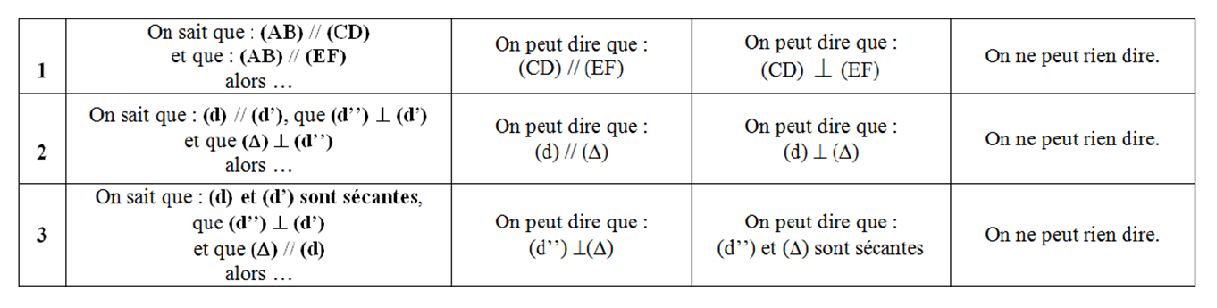
\includegraphics[scale=0.9]{qcm.eps} 
\end{flushleft}


\vspace*{0.5cm}

\exo{4} 
\includegraphics[scale=0.3]{trefle.eps} Écrire les codages manquants sur chacune des figures

\bmul{2}
\initq
\q On sait que : \\
 \noindent - O est le milieu de [AC],\\
 -  OB = OA \\
 - $(AB) \perp (BC)$


\columnbreak

\includegraphics[scale=1]{codage.eps} 

\emul

\newpage

\bmul{2}

\q  On sait que : \\
\noindent - PA = AR = RI = IS = SP\\
- US = UP = UA \\
- US = UR = UI



\columnbreak

\includegraphics[scale=0.8]{codage3.eps} 

\emul



\bmul{2}

\q On sait que : \\
\noindent - LP = PE = EL\\
 - ME = MU \\
 - $(LE) \perp (LM)$ \\
 - $(LM)  \perp (MU) $

\columnbreak

\includegraphics[scale=0.5]{codage1.eps} 

\emul




\exo{6} \\

\initq \q Sur votre copie double, en prenant soin de ne pas tracer sur les lignes, effectuer les constructions suivantes :\\
\initqa \qa	Tracer un segment [AB] de longueur 5,2 cm et placer son milieu C.\\
\qa	Sans utiliser les graduations de la règle, placer le point D pour que B soit le milieu de [AD].\\
\qa Tracer la médiatrice $(d_{1})$ du segment [AC].\\
\qa   Tracer la médiatrice  $(d_{2})$ du segment [BD].\\

\q Démontrer que les droites  $(d_{1})$ et $(d_{2})$ sont perpendiculaires.\\


\vspace*{0.5cm}

\exo{3} Calculer astucieusement en détaillant les étapes de calculs.\\



G = 1,4 + 75 + 18,60 + 125 + 2,9\\



 R = 5,125 + 21 + 4,7 + 9 + 2,3 + 0,875 + 34\\


\vspace*{0.5cm}

\exo{4}\\
Angèle et Élise ont reçu chacune la même somme d'argent de leur grand-mère.\\
Angèle, qui possédait 34,65 euros, a maintenant 100 euros. \\
Élise, quant à elle, possédait 48,50 euros.\\

\noindent \initq \q Combien d'argent leur grand-mère leur a-t-elle donné ? \\
\q Combien Élise a-t-elle d'argent maintenant ?\\

\vspace*{0.2cm}

\exo{} 
\includegraphics[scale=0.3]{trefle.eps} BONUS\\

\includegraphics[scale=1.1]{mediatrice3.eps} 




\end{document}
